\documentclass[aspectratio=169, ignorenonframetext]{beamer}
\usepackage{pgf}

\mode<article>{
  \usepackage{fullpage}

}

\mode<presentation>
{
  \usetheme{Madrid}
  \useinnertheme{circles}
  \setbeamertemplate{navigation symbols}{}
%   \usetheme[hideothersubsections, width=2.4cm]{Hannover}
%   \usetheme{Antibes}
%   \usetheme{Montpellier}
%   \usetheme{Singapore}
%   \usecolortheme{seahorse}
   \setbeamertemplate{footline}
   {%
%      \begin{beamercolorbox}{section in head/foot}
%       \usebeamercolor{bg}
%        \hskip 1em \footnotesize \insertframenumber{} / \inserttotalframenumber%\hskip 41em 
\includegraphics[height = .5cm]{../../bilder/cc_by-nc_eu.png}
%        
\includegraphics{../../bilder/cc_by-nc_eu.png}
% cc_by-nc_eu.png: 403x141 px, 72dpi, 14.22x4.97 cm, bb=0 0 403 141

% % cc_by-nc_eu.png: 403x141 px, 72dpi, 14.22x4.97 cm, bb=0 0 403 141
%
% % bwslogo_3.png: 476x392 px, 300dpi, 4.03x3.32 cm, bb=0 0 114 94
%
%       %\hskip 5em
%       %       \input{../bilder/cc_by.png}
%       %\includegraphics[height=.5cm]{../../../../bilder/bwslogo_3.png}
%      \end{beamercolorbox}%
   }
  \usepackage{beamerfoils}
}
\usepackage[utf8]{inputenc}
\usepackage[german]{babel}
\usepackage[utf8]{inputenc}
\usepackage{times}
\usepackage[T1]{fontenc}
\usepackage{eurosym}
\usepackage{graphicx}
\usepackage{amsmath}
\usepackage[siunitx,european]{circuitikz}
% \usepackage{ulem}
\usepackage{listings}
%
\lstset{numbers=left, numberstyle=\tiny, stepnumber=2, numbersep=5pt, language = C++, alsolanguage=XML}

\only<article>{
  \usepackage[colorlinks=true,linkcolor=blue,filecolor=magenta,urlcolor=cyan]{hyperref}
}

\only<presentation>{
% \MyLogo{\includegrapshics[height=1cm]{../../../../../bilder/bwslogo_3.png}}

  \usepackage{hyperref}
}


\title{Arbeitsunterlagen zu FOS Elektrotechnik Themenfeld 12.2}
\subtitle{Wechselstromtechnik}
% \date{Stand: \today}%\\

\institute[BWS Hofheim]{Brühlwiesenschule, Hofheim}
\author{Thomas Maul}

\titlegraphic{Für eigene Teile gilt: 
\includegraphics[height=1cm]{../../bilder/cc_by-nc_eu.png}}


\begin{document}

  \only<article>{
    \maketitle
    \tableofcontents
    \clearpage
  }
\begin{frame}<beamer>
  \titlepage
  % \hyperlink{Teil_2}{\beamerbutton{Go part 2}}
\end{frame}

\begin{frame}{Kondensator in Wechselspannung}
  \begin{itemize}
    \item Komplexer Widerstand
    \item steigende Frequenz $\rightarrow$ klinerer (Blind-)Widerstand
  \end{itemize}
\end{frame}

\begin{frame}{Spule in Wechselspannung}
  \begin{itemize}
    \item Komplexer Widerstand
    \item steigende Frequenz $\rightarrow$ größerer (Blind-)Widerstand
  \end{itemize}
\end{frame}

\begin{frame}{Vierpol oder Zweitor}
\begin{columns}
\begin{column}{.5\linewidth}
\begin{itemize}
 \item links Eingang ($\text{U}_e$), rechts Ausgang ($\text{U}_a$)
 \item Inhalt "`beliebig"'
 \item z. B. Schaltung von Widerständen, Spulen Kondensatoren, \dots
\end{itemize}
\end{column}
\begin{column}{.5\linewidth}
\begin{figure}
 \centering
 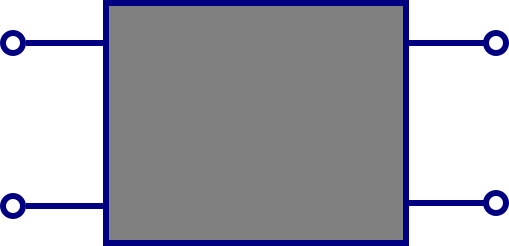
\includegraphics[scale = .5]{vierpolKasten.png}
 % vierpolKasten.png: 0x0 px, 0dpi, nanxnan cm, bb=
 \label{abb:VierpolKasten}
\end{figure}
\end{column}
\end{columns}
\end{frame}

\begin{frame}{Tiefpass}
\begin{columns}
\begin{column}{.5\linewidth}
\begin{itemize}
 \item Lässt tiefe Frequenzen passieren
 \item Grenzfrequenz = Abfall von 3\,dB (Ue/Ua)
 \item je höher Frequenz = geringerer Ausgang (Spannnung)
 \item Verscheibung der Phase! (Bei -3\,dB um 45 Grad)
\end{itemize}
\end{column}
\begin{column}{.5\linewidth}
\begin{figure}
 \centering
 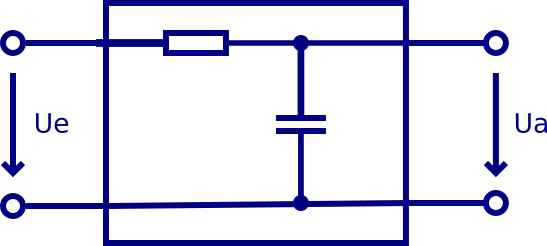
\includegraphics[scale = .5]{vierpolTP.png}
 % vierpolKasten.png: 0x0 px, 0dpi, nanxnan cm, bb=
 \label{abb:VierpolTP}
\end{figure}
\end{column}
\end{columns}
\href{https://de.wikipedia.org/wiki/Tiefpass}{\beamerbutton{TP bei Wikipedia}}
\end{frame}




\end{document}
